\documentclass[11pt,preprint]{elsarticle}

\usepackage{lmodern}
%%%% My spacing
\usepackage{setspace}
\setstretch{1.2}
\DeclareMathSizes{12}{14}{10}{10}

% Wrap around which gives all figures included the [H] command, or places it "here". This can be tedious to code in Rmarkdown.
\usepackage{float}
\let\origfigure\figure
\let\endorigfigure\endfigure
\renewenvironment{figure}[1][2] {
    \expandafter\origfigure\expandafter[H]
} {
    \endorigfigure
}

\let\origtable\table
\let\endorigtable\endtable
\renewenvironment{table}[1][2] {
    \expandafter\origtable\expandafter[H]
} {
    \endorigtable
}


\usepackage{ifxetex,ifluatex}
\usepackage{fixltx2e} % provides \textsubscript
\ifnum 0\ifxetex 1\fi\ifluatex 1\fi=0 % if pdftex
  \usepackage[T1]{fontenc}
  \usepackage[utf8]{inputenc}
\else % if luatex or xelatex
  \ifxetex
    \usepackage{mathspec}
    \usepackage{xltxtra,xunicode}
  \else
    \usepackage{fontspec}
  \fi
  \defaultfontfeatures{Mapping=tex-text,Scale=MatchLowercase}
  \newcommand{\euro}{€}
\fi

\usepackage{amssymb, amsmath, amsthm, amsfonts}

\def\bibsection{\section*{References}} %%% Make "References" appear before bibliography


\usepackage[numbers]{natbib}

\usepackage{longtable}
\usepackage[margin=2.3cm,bottom=2cm,top=2.5cm, includefoot]{geometry}
\usepackage{fancyhdr}
\usepackage[bottom, hang, flushmargin]{footmisc}
\usepackage{graphicx}
\numberwithin{equation}{section}
\numberwithin{figure}{section}
\numberwithin{table}{section}
\setlength{\parindent}{0cm}
\setlength{\parskip}{1.3ex plus 0.5ex minus 0.3ex}
\usepackage{textcomp}
\renewcommand{\headrulewidth}{0.2pt}
\renewcommand{\footrulewidth}{0.3pt}

\usepackage{array}
\newcolumntype{x}[1]{>{\centering\arraybackslash\hspace{0pt}}p{#1}}

%%%%  Remove the "preprint submitted to" part. Don't worry about this either, it just looks better without it:
\makeatletter
\def\ps@pprintTitle{%
  \let\@oddhead\@empty
  \let\@evenhead\@empty
  \let\@oddfoot\@empty
  \let\@evenfoot\@oddfoot
}
\makeatother

 \def\tightlist{} % This allows for subbullets!

\usepackage{hyperref}
\hypersetup{breaklinks=true,
            bookmarks=true,
            colorlinks=true,
            citecolor=blue,
            urlcolor=blue,
            linkcolor=blue,
            pdfborder={0 0 0}}


% The following packages allow huxtable to work:
\usepackage{siunitx}
\usepackage{multirow}
\usepackage{hhline}
\usepackage{calc}
\usepackage{tabularx}
\usepackage{booktabs}
\usepackage{caption}


\newenvironment{columns}[1][]{}{}

\newenvironment{column}[1]{\begin{minipage}{#1}\ignorespaces}{%
\end{minipage}
\ifhmode\unskip\fi
\aftergroup\useignorespacesandallpars}

\def\useignorespacesandallpars#1\ignorespaces\fi{%
#1\fi\ignorespacesandallpars}

\makeatletter
\def\ignorespacesandallpars{%
  \@ifnextchar\par
    {\expandafter\ignorespacesandallpars\@gobble}%
    {}%
}
\makeatother


% definitions for citeproc citations
\NewDocumentCommand\citeproctext{}{}
\NewDocumentCommand\citeproc{mm}{%
\href{\#cite.\detokenize{#1}}{#2}\nocite{#1}}

\makeatletter
% allow citations to break across lines
\let\@cite@ofmt\@firstofone
% avoid brackets around text for \cite:
\def\@biblabel#1{}
\def\@cite#1#2{{#1\if@tempswa , #2\fi}}
\makeatother
\newlength{\cslhangindent}
\setlength{\cslhangindent}{1.5em}
\newlength{\csllabelwidth}
\setlength{\csllabelwidth}{3em}
\newenvironment{CSLReferences}[2] % #1 hanging-indent, #2 entry-spacing
{\begin{list}{}{%
	\setlength{\itemindent}{0pt}
	\setlength{\leftmargin}{0pt}
	\setlength{\parsep}{0pt}
	% turn on hanging indent if param 1 is 1
	\ifodd #1
	\setlength{\leftmargin}{\cslhangindent}
	\setlength{\itemindent}{-1\cslhangindent}
	\fi
	% set entry spacing
	\setlength{\itemsep}{#2\baselineskip}}}
{\end{list}}

\usepackage{calc}
\newcommand{\CSLBlock}[1]{\hfill\break\parbox[t]{\linewidth}{\strut\ignorespaces#1\strut}}
\newcommand{\CSLLeftMargin}[1]{\parbox[t]{\csllabelwidth}{\strut#1\strut}}
\newcommand{\CSLRightInline}[1]{\parbox[t]{\linewidth - \csllabelwidth}{\strut#1\strut}}
\newcommand{\CSLIndent}[1]{\hspace{\cslhangindent}#1}


\urlstyle{same}  % don't use monospace font for urls
\setlength{\parindent}{0pt}
\setlength{\parskip}{6pt plus 2pt minus 1pt}
\setlength{\emergencystretch}{3em}  % prevent overfull lines
\setcounter{secnumdepth}{5}

%%% Use protect on footnotes to avoid problems with footnotes in titles
\let\rmarkdownfootnote\footnote%
\def\footnote{\protect\rmarkdownfootnote}
\IfFileExists{upquote.sty}{\usepackage{upquote}}{}

%%% Include extra packages specified by user

%%% Hard setting column skips for reports - this ensures greater consistency and control over the length settings in the document.
%% page layout
%% paragraphs
\setlength{\baselineskip}{12pt plus 0pt minus 0pt}
\setlength{\parskip}{12pt plus 0pt minus 0pt}
\setlength{\parindent}{0pt plus 0pt minus 0pt}
%% floats
\setlength{\floatsep}{12pt plus 0 pt minus 0pt}
\setlength{\textfloatsep}{20pt plus 0pt minus 0pt}
\setlength{\intextsep}{14pt plus 0pt minus 0pt}
\setlength{\dbltextfloatsep}{20pt plus 0pt minus 0pt}
\setlength{\dblfloatsep}{14pt plus 0pt minus 0pt}
%% maths
\setlength{\abovedisplayskip}{12pt plus 0pt minus 0pt}
\setlength{\belowdisplayskip}{12pt plus 0pt minus 0pt}
%% lists
\setlength{\topsep}{10pt plus 0pt minus 0pt}
\setlength{\partopsep}{3pt plus 0pt minus 0pt}
\setlength{\itemsep}{5pt plus 0pt minus 0pt}
\setlength{\labelsep}{8mm plus 0mm minus 0mm}
\setlength{\parsep}{\the\parskip}
\setlength{\listparindent}{\the\parindent}
%% verbatim
\setlength{\fboxsep}{5pt plus 0pt minus 0pt}



\begin{document}



\begin{frontmatter}  %

\title{Question\_1}

% Set to FALSE if wanting to remove title (for submission)




\author[Add1]{Happy Matope}
\ead{your-student-number@sun.ac.za}





\address[Add1]{Stellenbosch University, South Africa}



\vspace{1cm}


\begin{keyword}
\footnotesize{
Realised volatility \sep GJR-GARCH \sep DCC \sep Risk contribution
\sep Factor exposure \sep Dispersion \\
\vspace{0.3cm}
}
\footnotesize{
\textit{JEL classification} G11 \sep G12 \sep C58
}
\end{keyword}



\vspace{0.5cm}

\end{frontmatter}

\setcounter{footnote}{0}



%________________________
% Header and Footers
%%%%%%%%%%%%%%%%%%%%%%%%%%%%%%%%%
\pagestyle{fancy}
\chead{}
\rhead{Offshore Uncertainty, Local Volatility and the Case for Risk
Ballasts}
\lfoot{}
\rfoot{\footnotesize Page \thepage}
\lhead{}
%\rfoot{\footnotesize Page \thepage } % "e.g. Page 2"
\cfoot{}

%\setlength\headheight{30pt}
%%%%%%%%%%%%%%%%%%%%%%%%%%%%%%%%%
%________________________

\headsep 35pt % So that header does not go over title




\makeatletter
\@ifundefined{pandocbounded}{%
  \newsavebox\pandoc@box
  \newcommand*\pandocbounded[1]{%
    \sbox\pandoc@box{#1}%
    \Gscale@div\@tempa{\textheight}{\dimexpr\ht\pandoc@box+\dp\pandoc@box\relax}%
    \Gscale@div\@tempb{\linewidth}{\wd\pandoc@box}%
    \ifdim\@tempb\p@<\@tempa\p@\let\@tempa\@tempb\fi
    \ifdim\@tempa\p@<\p@\scalebox{\@tempa}{\usebox\pandoc@box}%
    \else\usebox{\pandoc@box}\fi}%
}{}
\makeatother

\section{\texorpdfstring{Introduction
\label{Introduction}}{Introduction }}\label{introduction}

Oil-price swings and global policy uncertainty have dominated recent
market commentary. For a team managing local equity funds, the practical
question is whether this offshore uncertainty is spilling into South
African equity volatility. If it is, should funds hold more ``risk
ballast'': stocks or tilts that dampen volatility when global stress
rises?

This report answers that question in three parts.

\begin{itemize}
\tightlist
\item
  \textbf{Part A} asks whether volatility on the JSE has increased, and
  whether it mirrors the global experience. It uses realised volatility,
  GARCH and DCC models, and stratification by global uncertainty
  measures.
\item
  \textbf{Part B} evaluates whether the firm's SafeCore portfolio, which
  is not built with volatility in mind, handles volatility well. It also
  asks where SafeCore's risk comes from and what its factor exposures
  are, using our own momentum and low-volatility scores alongside a
  third party's.
\item
  \textbf{Part C} measures the alpha opportunity in the local market
  since 2020, using cross-sectional dispersion and inter-stock
  correlation, and links it to global macro conditions.
\end{itemize}

Section \ref{Data} describes the data, Section \ref{Method} the methods,
Section \ref{Results} the results, and Section \ref{Summary} summarises.

\section{\texorpdfstring{Data \label{Data}}{Data }}\label{data}

Table \ref{tab:data} lists the data.

\begin{itemize}
\tightlist
\item
  \textbf{Local market:} the Capped SWIX (J433), the fund's benchmark,
  and the Top 40 (J200), as daily returns from January 2015.
\item
  \textbf{Global comparison:} the MSCI World and MSCI Emerging Markets
  total return indexes, in US dollars.
\item
  \textbf{SafeCore:} the portfolio's month-end holdings. Combined with
  daily stock returns, they rebuild its daily returns.
\item
  \textbf{Factor scores:} a third party's monthly scores (2020 onwards)
  for earnings quality, growth, momentum, value and volatility
  sensitivity.
\item
  \textbf{Offshore uncertainty:} implied volatility indexes (VIX, VXEEM,
  MOVE), economic policy uncertainty indexes, rand and global currency
  volatility, and Brent crude.
\end{itemize}

\begin{verbatim}
tab_print(Tab_Data, caption = "Data used", label = "tab:data", size = "\\scriptsize")
\end{verbatim}

\begin{table}[!htbp]
\centering
\caption{Data used} 
\label{tab:data}
\begingroup\scriptsize
\begin{tabular}{lllll}
  \hline
Data & Frequency & Start & End & Coverage \\ 
  \hline
Local index returns (J433, J200, factor indexes) & Daily & Jan 2015 & Sep 2026 & Benchmark and context \\ 
  MSCI World and EM (USD TRI) & Daily & Jan 2005 & Sep 2026 & Global comparison \\ 
  SafeCore holdings & Monthly & Jan 2007 & Aug 2026 & Avg. 42 stocks \\ 
  Capped SWIX constituents \& weights & Monthly & Jan 2007 & Aug 2026 & Benchmark weights \\ 
  Daily stock returns & Daily & Jan 2015 & Sep 2026 & 277 stocks \\ 
  Third-party factor scores & Monthly & Jan 2020 & Aug 2026 & 5 factors \\ 
  Implied vol, policy uncertainty, currency vol, oil & Daily / monthly & Jan 2005 & Sep 2026 & 10 series \\ 
   \hline
\end{tabular}
\endgroup
\end{table}

Four data treatments matter.

\begin{itemize}
\tightlist
\item
  \textbf{Log returns are used for volatility work.} Simple returns are
  used for portfolio returns.
\item
  \textbf{Daily stock returns contain a few extreme values} (from
  \(-100\%\) to \(+900\%\) days on illiquid names). They are capped at
  \(\pm 25\%\) for volatility and factor scores, at \(\pm 50\%\) for
  dispersion (as in the course's dispersion practical), and cleaned with
  Boudt's method for risk contributions.
\item
  \textbf{SafeCore's weights sum to between 0.79 and 1.} They are
  rescaled each month, so the portfolio is treated as fully invested in
  equities.
\item
  \textbf{The policy-uncertainty indexes are monthly numbers repeated
  daily.} All driver series are therefore analysed at monthly frequency.
\end{itemize}

Table \ref{tab:desc} shows that local and global returns are all
negatively skewed and fat-tailed, and normality is rejected for each.
The fat tails motivate Student-\(t\) errors in the GARCH models. Table
\ref{tab:drivers} summarises the monthly driver series.

\begin{verbatim}
tab_print(Tab_Desc, caption = "Descriptive statistics of daily log returns (Jan 2015 to Sep 2026)",
          label = "tab:desc")
\end{verbatim}

\begin{table}[!htbp]
\centering
\caption{Descriptive statistics of daily log returns (Jan 2015 to Sep 2026)} 
\label{tab:desc}
\begingroup\footnotesize
\begin{tabular}{lrrrrrrrr}
  \hline
Series & Obs & Mean (ann.) & SD (ann.) & Skewness & Excess kurtosis & Min & Max & JB p-value \\ 
  \hline
J200 & 2935 & 0.105 & 0.188 & -0.455 & 5.829 & -0.105 & 0.079 & 0.000 \\ 
  J433 & 2935 & 0.083 & 0.179 & -0.591 & 7.335 & -0.096 & 0.067 & 0.000 \\ 
  MSCI EM & 3064 & 0.074 & 0.166 & -0.460 & 5.382 & -0.082 & 0.064 & 0.000 \\ 
  MSCI World & 3064 & 0.108 & 0.148 & -0.981 & 16.867 & -0.104 & 0.084 & 0.000 \\ 
   \hline
\end{tabular}
\endgroup
\end{table}

\begin{verbatim}
tab_print(Tab_Drivers, caption = "Monthly driver series (monthly averages, 2015 to 2026)",
          label = "tab:drivers", digits = 2)
\end{verbatim}

\begin{table}[!htbp]
\centering
\caption{Monthly driver series (monthly averages, 2015 to 2026)} 
\label{tab:drivers}
\begingroup\footnotesize
\begin{tabular}{lrrrrr}
  \hline
Series & Months & Mean & SD & Min & Max \\ 
  \hline
EPUCCEUM & 141 & 282.93 & 109.23 & 132.27 & 772.83 \\ 
  EPUCGLCP & 141 & 228.31 & 87.22 & 99.50 & 617.15 \\ 
  EPUCNUSD & 141 & 164.04 & 114.02 & 50.29 & 560.88 \\ 
  JPMVXYGL & 141 & 8.51 & 1.50 & 5.53 & 12.35 \\ 
  MOVE\_Index & 141 & 79.48 & 25.77 & 41.83 & 151.91 \\ 
  Oil\_Brent & 141 & 68.00 & 18.15 & 26.85 & 117.50 \\ 
  SAVIUSD & 141 & 14.86 & 3.44 & 0.14 & 21.36 \\ 
  V2X & 141 & 22.62 & 6.96 & 13.98 & 63.70 \\ 
  VIX & 141 & 18.31 & 6.33 & 10.13 & 57.74 \\ 
  VXEEM & 141 & 22.23 & 5.97 & 14.77 & 56.36 \\ 
   \hline
\end{tabular}
\endgroup
\end{table}

\section{\texorpdfstring{Methodology
\label{Method}}{Methodology }}\label{methodology}

\subsection{Realised volatility and
stratification}\label{realised-volatility-and-stratification}

With daily log returns \(r_t = \ln(1+R_t)\), realised volatility over a
window of \(n\) days is

\[
\sigma^{RV}_t = \sqrt{252}\cdot \text{sd}(r_{t-n+1},\dots,r_t),
\]

with \(n = 252\) for rolling one-year volatility.

For stratification, each month \(m\) is classified by a driver \(X_m\)
as ``High'' (top quintile) or ``Low'' (bottom quintile). A statistic,
such as J433 realised volatility, is then compared between the two
groups, using a Welch two-sample \(t\)-test. Because months are not
independent, the \(p\)-values are indicative.

\subsection{GJR-GARCH and EGARCH with external
regressors}\label{gjr-garch-and-egarch-with-external-regressors}

Conditional volatility is modelled with an AR(1) mean and a
GJR-GARCH(1,1) variance
(\citeproc{ref-glosten1993}{\textbf{glosten1993?}}):

\[
r_t = \mu + \phi r_{t-1} + \varepsilon_t,\quad \varepsilon_t = \sigma_t z_t,\quad z_t \sim t_\nu,
\qquad
\sigma_t^2 = \omega + (\alpha + \gamma I_{t-1})\varepsilon_{t-1}^2 + \beta\sigma_{t-1}^2.
\]

Here \(I_{t-1} = 1\) when \(\varepsilon_{t-1} < 0\). A positive
\(\gamma\) means bad news raises volatility more than good news (the
leverage effect). Persistence is \(\alpha + \beta + \gamma/2\).

The specification is chosen by information criteria from sGARCH,
GJR-GARCH, EGARCH and apARCH models.

To test whether offshore fear raises local volatility directly, an
EGARCH model includes lagged, standardised log VIX and log global policy
uncertainty, \(x_{t-1}\), in the variance equation:

\[
\ln\sigma_t^2 = \omega + \alpha z_{t-1} + \gamma\left(|z_{t-1}| - E|z_{t-1}|\right) + \beta\ln\sigma_{t-1}^2 + \delta' x_{t-1}.
\]

Because EGARCH models the log of the variance, the regressors cannot
push the variance negative.

\subsection{Dynamic conditional
correlation}\label{dynamic-conditional-correlation}

Time-varying correlation between J433 and global markets is estimated
with a DCC(1,1) model (\citeproc{ref-engle2002}{\textbf{engle2002?}}) on
weekly returns. Weekly data avoid the bias from the JSE and US markets
closing at different times. After fitting a GJR-GARCH to each series,
the standardised residuals \(u_t\) drive

\[
Q_t = (1-a-b)\bar{Q} + a\,u_{t-1}u_{t-1}' + b\,Q_{t-1},
\qquad
R_t = \text{diag}(Q_t)^{-1/2}\,Q_t\,\text{diag}(Q_t)^{-1/2}.
\]

A multivariate ARCH test first checks that the correlations are not
constant.

\subsection{Portfolio returns and risk
contributions}\label{portfolio-returns-and-risk-contributions}

SafeCore's daily return is \(R_{p,t} = \sum_i w_{i,t-1}R_{i,t}\), built
from month-end weights that drift within the month.

Each stock's share of portfolio risk uses Euler's decomposition. For a
risk measure \(\rho(w)\) that scales with the portfolio (such as SD or
Expected Shortfall),

\[
\rho(w) = \sum_i w_i \frac{\partial\rho(w)}{\partial w_i},
\qquad
\text{\% contribution}_i = \frac{w_i\,\partial\rho/\partial w_i}{\rho(w)}.
\]

For the SD,
\(w_i\,\partial\sigma_p/\partial w_i = w_i(\Sigma w)_i/\sigma_p\).
Contributions are computed with \texttt{PerformanceAnalytics}
(\texttt{ETL} and \texttt{StdDev},
\texttt{portfolio\_method\ =\ "component"}), as in the course's risk
practical.

\subsection{Factor scores and
exposures}\label{factor-scores-and-exposures}

Two of our own scores are built from price behaviour, for each Capped
SWIX constituent at each month-end:

\begin{itemize}
\tightlist
\item
  \textbf{Momentum} is the return over months \(t-5\) to \(t-1\): six
  months, skipping the latest month to avoid short-term reversal.
\item
  \textbf{Low volatility} is minus the annualised SD of the last 126
  daily returns.
\end{itemize}

Each score is standardised across constituents and capped at \(\pm 3\):
\(z_{i,t} = \min(\max((x_{i,t}-\bar{x}_t)/s_t, -3), 3)\).

Agreement with the third party's scores is measured by the monthly
Spearman rank correlation.

A portfolio's exposure to a factor is its weighted average score,
\(E_t = \sum_i w_{i,t}z_{i,t}\). Active exposure is SafeCore's exposure
minus the Capped SWIX's.

Composite strategy scores average the relevant \(z\)-scores. SafeCore's
``purity'' for each strategy measures how far it sits from the benchmark
towards a pure strategy portfolio (the equal-weighted top quintile of
the score):

\[
\text{Purity}_t = \frac{E^{SC}_t - E^{J433}_t}{E^{\text{Top}}_t - E^{J433}_t}.
\]

\subsection{Dispersion and
correlation}\label{dispersion-and-correlation}

Following the course's dispersion practical, the weighted
cross-sectional volatility of the Capped SWIX constituents uses rolling
\(n\)-week returns \(R_{i,t}\) and the previous month-end weights:

\[
\text{CSV}^{W}_t = \sqrt{\sum_i w_{i,t}\,(R_{i,t} - R_{J433,t})^2}.
\]

The unweighted version uses equal weights around the equal-weighted
mean.

Co-movement is measured each month-end among the 40 largest stocks, over
the last 63 trading days, in two ways:

\begin{itemize}
\tightlist
\item
  the average pairwise correlation;
\item
  the share of variance explained by the first principal component of
  the correlation matrix, \(\lambda_1/\sum_k\lambda_k\).
\end{itemize}

High dispersion with low correlation marks the best environment for
stock pickers.

\section{\texorpdfstring{Results
\label{Results}}{Results }}\label{results}

\subsection{Part A: Has local volatility increased, and does it mirror
the global
experience?}\label{part-a-has-local-volatility-increased-and-does-it-mirror-the-global-experience}

\subsubsection{Realised volatility}\label{realised-volatility}

Local volatility is not structurally higher than before 2020, but it has
risen again in 2026 (Table \ref{tab:volperiod}, Figure \ref{FigA1}).

\begin{itemize}
\tightlist
\item
  \textbf{The Capped SWIX's realised volatility was about 16\%} in
  2015--19 and again in 2024--26, after peaking at 31\% in 2020.
\item
  \textbf{Within 2026 it has jumped:} 20.7\% so far this year, against
  15.0\% in 2025 (Table \ref{tab:volyear}).
\item
  \textbf{The global experience is split.} Emerging-market volatility
  has risen to 25\% in 2026, while developed-market (MSCI World)
  volatility has stayed low at about 12\%.
\end{itemize}

\begin{verbatim}
tab_print(Vol_Periods, caption = "Annualised realised volatility by period (daily log returns)",
          label = "tab:volperiod")
\end{verbatim}

\begin{table}[!htbp]
\centering
\caption{Annualised realised volatility by period (daily log returns)} 
\label{tab:volperiod}
\begingroup\footnotesize
\begin{tabular}{lrrrr}
  \hline
Tickers & 1. 2015-2019 & 2. 2020 (Covid) & 3. 2021-2023 & 4. 2024-2026 \\ 
  \hline
J200 (Top 40) & 0.163 & 0.304 & 0.190 & 0.170 \\ 
  J433 (Capped SWIX) & 0.160 & 0.308 & 0.166 & 0.160 \\ 
  MXEF Index (MSCI\_EM) & 0.141 & 0.237 & 0.163 & 0.180 \\ 
  MXWO Index (MSCI\_AllWorld) & 0.112 & 0.289 & 0.151 & 0.126 \\ 
   \hline
\end{tabular}
\endgroup
\end{table}

\begin{verbatim}
fmxdat::finplot(g_roll, x.date.dist = "1 year", x.date.type = "%Y",
                x.vert = TRUE, y.pct = TRUE, y.pct_acc = 1)
\end{verbatim}

\begin{figure}
\centering
\pandocbounded{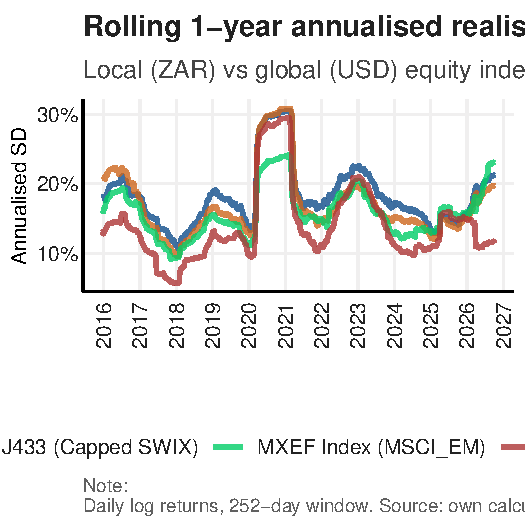
\includegraphics[keepaspectratio,alt={Rolling one-year realised volatility: local versus global }]{Question1_files/figure-latex/FigA1-1.pdf}}
\caption{Rolling one-year realised volatility: local versus global
\label{FigA1}}
\end{figure}

\begin{verbatim}
tab_print(Vol_Yearly %>% mutate(Year = as.character(Year)),
          caption = "Annualised realised volatility by calendar year (2026 = Jan to Sep)",
          label = "tab:volyear", size = "\\scriptsize")
\end{verbatim}

\begin{table}[!htbp]
\centering
\caption{Annualised realised volatility by calendar year (2026 = Jan to Sep)} 
\label{tab:volyear}
\begingroup\scriptsize
\begin{tabular}{lrrrr}
  \hline
Year & J200 (Top 40) & J433 (Capped SWIX) & MXEF Index (MSCI\_EM) & MXWO Index (MSCI\_AllWorld) \\ 
  \hline
2015 & 0.183 & 0.208 & 0.160 & 0.130 \\ 
  2016 & 0.182 & 0.176 & 0.169 & 0.127 \\ 
  2017 & 0.112 & 0.096 & 0.093 & 0.057 \\ 
  2018 & 0.187 & 0.165 & 0.153 & 0.126 \\ 
  2019 & 0.139 & 0.130 & 0.114 & 0.101 \\ 
  2020 & 0.304 & 0.308 & 0.237 & 0.289 \\ 
  2021 & 0.169 & 0.146 & 0.149 & 0.111 \\ 
  2022 & 0.225 & 0.196 & 0.202 & 0.207 \\ 
  2023 & 0.172 & 0.152 & 0.129 & 0.113 \\ 
  2024 & 0.132 & 0.123 & 0.131 & 0.108 \\ 
  2025 & 0.157 & 0.150 & 0.157 & 0.148 \\ 
  2026 & 0.224 & 0.207 & 0.251 & 0.119 \\ 
   \hline
\end{tabular}
\endgroup
\end{table}

Local volatility mirrors global volatility closely, but more closely EM
than the developed world.

\begin{itemize}
\tightlist
\item
  \textbf{The rolling-volatility paths move together}: J433 correlates
  0.89 with MSCI World and 0.91 with MSCI EM (Table \ref{tab:volcor}).
\item
  \textbf{The local market is consistently more volatile than the
  developed world}, and roughly as volatile as other emerging markets
  (Figure \ref{FigA2}, Table \ref{tab:relvol}).
\end{itemize}

\begin{verbatim}
tab_print(as_tibble(Vol_Path_Cor, rownames = "Series"),
          caption = "Correlation between rolling one-year volatility paths (month-end)",
          label = "tab:volcor", size = "\\scriptsize")
\end{verbatim}

\begin{table}[!htbp]
\centering
\caption{Correlation between rolling one-year volatility paths (month-end)} 
\label{tab:volcor}
\begingroup\scriptsize
\begin{tabular}{lrrrr}
  \hline
Series & MXWO Index (MSCI\_AllWorld) & MXEF Index (MSCI\_EM) & J433 (Capped SWIX) & J200 (Top 40) \\ 
  \hline
MXWO Index (MSCI\_AllWorld) & 1.000 & 0.856 & 0.895 & 0.915 \\ 
  MXEF Index (MSCI\_EM) & 0.856 & 1.000 & 0.905 & 0.907 \\ 
  J433 (Capped SWIX) & 0.895 & 0.905 & 1.000 & 0.970 \\ 
  J200 (Top 40) & 0.915 & 0.907 & 0.970 & 1.000 \\ 
   \hline
\end{tabular}
\endgroup
\end{table}

\begin{verbatim}
fmxdat::finplot(g_rel, x.date.dist = "1 year", x.date.type = "%Y", x.vert = TRUE)
\end{verbatim}

\begin{figure}
\centering
\pandocbounded{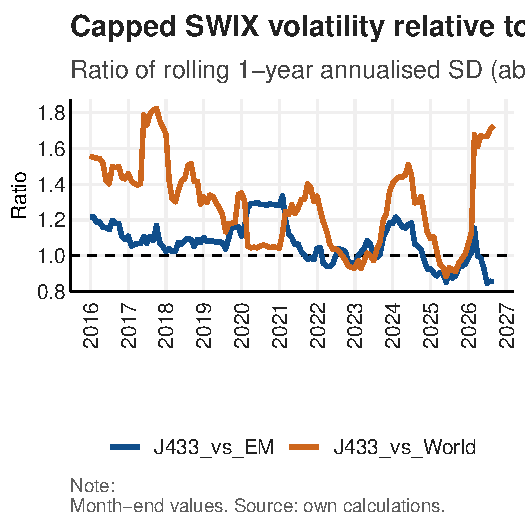
\includegraphics[keepaspectratio,alt={Capped SWIX volatility relative to global volatility }]{Question1_files/figure-latex/FigA2-1.pdf}}
\caption{Capped SWIX volatility relative to global volatility
\label{FigA2}}
\end{figure}

\begin{verbatim}
tab_print(Rel_Summary, caption = "Average ratio of J433 volatility to global volatility",
          label = "tab:relvol", digits = 2)
\end{verbatim}

\begin{table}[!htbp]
\centering
\caption{Average ratio of J433 volatility to global volatility} 
\label{tab:relvol}
\begingroup\footnotesize
\begin{tabular}{lrrrr}
  \hline
Ratio & 1. 2015-2019 & 2. 2020 & 3. 2021-2023 & 4. 2024-2026 \\ 
  \hline
J433\_vs\_EM & 1.10 & 1.26 & 1.04 & 1.00 \\ 
  J433\_vs\_World & 1.45 & 1.10 & 1.13 & 1.27 \\ 
   \hline
\end{tabular}
\endgroup
\end{table}

\subsubsection{GARCH volatility and dynamic
correlation}\label{garch-volatility-and-dynamic-correlation}

Volatility clusters strongly: the Ljung--Box test on squared J433
returns rejects ``no ARCH effects'' decisively (Table \ref{tab:diag}).

Among the four GARCH variants (Table \ref{tab:fit}), the two asymmetric
models clearly beat the standard GARCH. EGARCH has a marginally lower
AIC than GJR-GARCH (by 0.005), a negligible difference. GJR-GARCH is
retained because, as in the course practical, its parameters are easier
to interpret.

\begin{verbatim}
tab_print(Fit_Tab, caption = "Information criteria for J433 (lower is better)", label = "tab:fit")
\end{verbatim}

\begin{table}[!htbp]
\centering
\caption{Information criteria for J433 (lower is better)} 
\label{tab:fit}
\begingroup\footnotesize
\begin{tabular}{lrrrr}
  \hline
Criterion & sGARCH & gjrGARCH & eGARCH & apARCH \\ 
  \hline
Akaike & -6.394 & -6.410 & -6.415 & -6.402 \\ 
  Bayes & -6.382 & -6.395 & -6.400 & -6.385 \\ 
  Shibata & -6.394 & -6.410 & -6.415 & -6.402 \\ 
  Hannan-Quinn & -6.390 & -6.405 & -6.409 & -6.396 \\ 
   \hline
\end{tabular}
\endgroup
\end{table}

Table \ref{tab:garch} gives the GJR-GARCH estimates.

\begin{itemize}
\tightlist
\item
  \textbf{Volatility reacts almost only to bad news.} \(\alpha\) is
  close to zero and insignificant, while \(\gamma\) is large and
  significant for all three markets.
\item
  \textbf{The local market is less asymmetric than global markets}
  (\(\gamma\) = 0.13 against 0.23 for MSCI World).
\item
  \textbf{Local shocks fade with a half-life of about 20 trading days},
  slower than EM and faster than MSCI World.
\item
  \textbf{Fat tails are confirmed} by Student-\(t\) shape parameters of
  about 6--9.
\end{itemize}

The diagnostics are acceptable (Table \ref{tab:diag}). No ARCH effects
remain in the squared standardised residuals (\(p\) = 0.98), and the
sign-bias test suggests the asymmetry is largely captured (\(p\) =
0.06).

\begin{verbatim}
tab_print(Garch_Tab, caption = "GJR-GARCH(1,1) estimates: AR(1) mean, Student-t errors",
          label = "tab:garch", size = "\\scriptsize")
\end{verbatim}

\begin{table}[!htbp]
\centering
\caption{GJR-GARCH(1,1) estimates: AR(1) mean, Student-t errors} 
\label{tab:garch}
\begingroup\scriptsize
\begin{tabular}{lrrrrrrrr}
  \hline
Series & alpha & alpha p & beta & gamma & gamma p & shape & Persistence & Half-life (days) \\ 
  \hline
J433 & 0.005 & 0.265 & 0.899 & 0.126 & 0.000 & 6.712 & 0.966 & 20.324 \\ 
  MSCI\_World & 0.000 & 0.995 & 0.862 & 0.234 & 0.000 & 5.953 & 0.979 & 32.261 \\ 
  MSCI\_EM & 0.014 & 0.012 & 0.839 & 0.185 & 0.000 & 8.619 & 0.946 & 12.399 \\ 
   \hline
\end{tabular}
\endgroup
\end{table}

\begin{verbatim}
tab_print(Diag_Tab, caption = "Diagnostic tests (J433)", label = "tab:diag")
\end{verbatim}

\begin{table}[!htbp]
\centering
\caption{Diagnostic tests (J433)} 
\label{tab:diag}
\begingroup\footnotesize
\begin{tabular}{lrr}
  \hline
Test & Statistic & p-value \\ 
  \hline
Ljung-Box, squared returns (ARCH effects) & 2594.951 & 0.000 \\ 
  Ljung-Box, standardised residuals & 21.035 & 0.050 \\ 
  Ljung-Box, squared standardised residuals & 4.114 & 0.981 \\ 
  Sign bias: joint effect & 7.423 & 0.060 \\ 
   \hline
\end{tabular}
\endgroup
\end{table}

Conditional volatility (Figure \ref{FigA3}) tells the same story as
realised volatility. Since 2024, local volatility has resembled EM
(about 16\%) more than the developed world (about 12\%). The news impact
curve (Figure \ref{FigA4}) shows the asymmetry directly: a negative
shock raises next-day variance far more than a positive shock of the
same size.

\begin{verbatim}
fmxdat::finplot(g_sigma, x.date.dist = "1 year", x.date.type = "%Y",
                x.vert = TRUE, y.pct = TRUE, y.pct_acc = 1)
\end{verbatim}

\begin{figure}
\centering
\pandocbounded{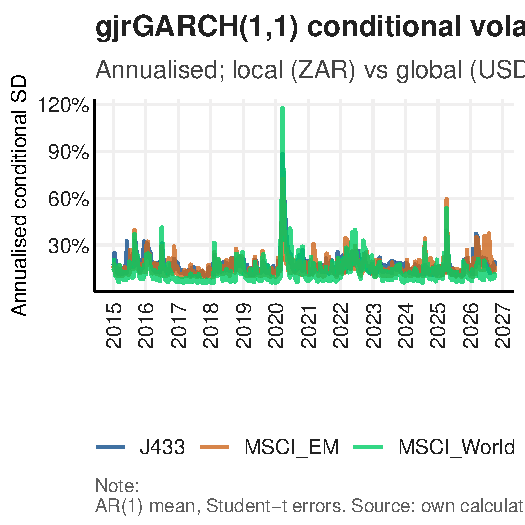
\includegraphics[keepaspectratio,alt={GJR-GARCH(1,1) conditional volatility }]{Question1_files/figure-latex/FigA3-1.pdf}}
\caption{GJR-GARCH(1,1) conditional volatility \label{FigA3}}
\end{figure}

\begin{verbatim}
fmxdat::finplot(g_ni)
\end{verbatim}

\begin{figure}
\centering
\pandocbounded{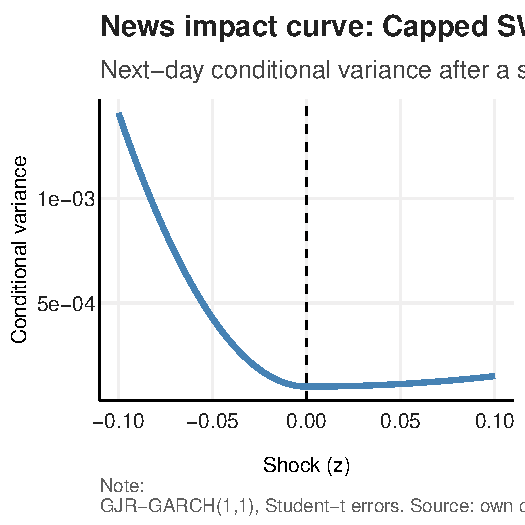
\includegraphics[keepaspectratio,alt={News impact curve for the Capped SWIX }]{Question1_files/figure-latex/FigA4-1.pdf}}
\caption{News impact curve for the Capped SWIX \label{FigA4}}
\end{figure}

Offshore fear raises local volatility directly (Table \ref{tab:vx}).

\begin{itemize}
\tightlist
\item
  \textbf{VIX:} in the EGARCH model with external regressors,
  yesterday's VIX has a positive and highly significant effect on the
  local conditional variance.
\item
  \textbf{Global policy uncertainty:} its effect is small and negative.
\item
  \textbf{Model fit:} adding the two regressors improves the AIC from
  -6.415 to -6.422.
\end{itemize}

So market-based fear (VIX) matters for local volatility; slow-moving
policy uncertainty does not add to it.

\begin{verbatim}
tab_print(VX_Tab, caption = "EGARCH(1,1) with external regressors in the variance equation (J433)",
          label = "tab:vx")
\end{verbatim}

\begin{table}[!htbp]
\centering
\caption{EGARCH(1,1) with external regressors in the variance equation (J433)} 
\label{tab:vx}
\begingroup\footnotesize
\begin{tabular}{lrrr}
  \hline
Parameter & Estimate & Std. Error & p-value \\ 
  \hline
alpha1 & -0.121 & 0.016 & 0.000 \\ 
  gamma1 & 0.132 & 0.022 & 0.000 \\ 
  beta1 & 0.912 & 0.010 & 0.000 \\ 
  VIX (lagged) & 0.042 & 0.003 & 0.000 \\ 
  Global EPU (lagged) & -0.013 & 0.005 & 0.006 \\ 
   \hline
\end{tabular}
\endgroup
\end{table}

The DCC model (Table \ref{tab:dcc}, Figure \ref{FigA5}) shows how
co-movement behaves over time.

\begin{itemize}
\tightlist
\item
  \textbf{Correlations are time-varying.} The multivariate ARCH tests
  reject constant correlation.
\item
  \textbf{They are persistent:} \(b\) = 0.93.
\item
  \textbf{Their long-run level has barely changed.} J433's average
  correlation with EM was 0.68 in 2015--19 and 0.69 in 2020--26, and
  0.64 against 0.66 with MSCI World (Table \ref{tab:dccper}).
\item
  \textbf{Correlations spike in crises}, most clearly to about 0.76 in
  March 2020 and again in April 2025. Global diversification therefore
  weakens exactly when it is most needed.
\end{itemize}

\begin{verbatim}
tab_print(DCC_Tab, caption = "DCC(1,1) correlation parameters (weekly returns)", label = "tab:dcc")
\end{verbatim}

\begin{table}[!htbp]
\centering
\caption{DCC(1,1) correlation parameters (weekly returns)} 
\label{tab:dcc}
\begingroup\footnotesize
\begin{tabular}{lrr}
  \hline
Parameter & Estimate & p-value \\ 
  \hline
a (dcca1) & 0.012 & 0.111 \\ 
  b (dccb1) & 0.932 & 0.000 \\ 
   \hline
\end{tabular}
\endgroup
\end{table}

\begin{verbatim}
fmxdat::finplot(g_dcc, x.date.dist = "1 year", x.date.type = "%Y", x.vert = TRUE)
\end{verbatim}

\begin{figure}
\centering
\pandocbounded{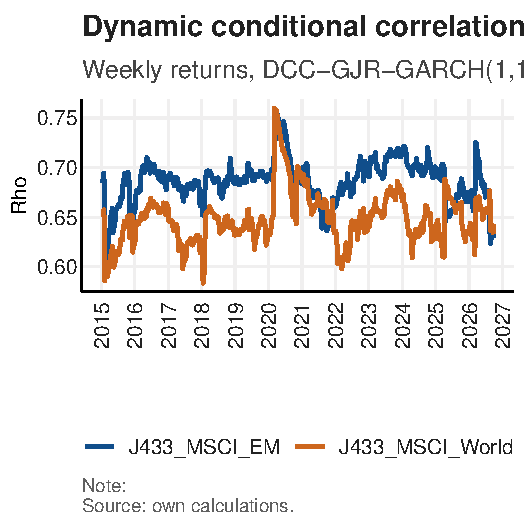
\includegraphics[keepaspectratio,alt={Dynamic conditional correlation of the Capped SWIX with global markets }]{Question1_files/figure-latex/FigA5-1.pdf}}
\caption{Dynamic conditional correlation of the Capped SWIX with global
markets \label{FigA5}}
\end{figure}

\begin{verbatim}
tab_print(DCC_Periods, caption = "Average dynamic correlation by period", label = "tab:dccper")
\end{verbatim}

\begin{table}[!htbp]
\centering
\caption{Average dynamic correlation by period} 
\label{tab:dccper}
\begingroup\footnotesize
\begin{tabular}{lrr}
  \hline
Pairs & 2015-2019 & 2020-2026 \\ 
  \hline
J433\_MSCI\_EM & 0.681 & 0.689 \\ 
  J433\_MSCI\_World & 0.637 & 0.656 \\ 
   \hline
\end{tabular}
\endgroup
\end{table}

\subsection{PART 3}\label{part-3}

\subsubsection{Does offshore uncertainty drive local
volatility?}\label{does-offshore-uncertainty-drive-local-volatility}

Global fear gauges and oil volatility track local volatility closely;
policy-uncertainty indexes do not (Table \ref{tab:unccor}, Figure
\ref{FigA6}).

\begin{itemize}
\tightlist
\item
  \textbf{Strong co-movers:} monthly J433 realised volatility correlates
  0.77 with EM implied volatility (VXEEM), 0.75 with the VIX and 0.71
  with oil volatility.
\item
  \textbf{Weak co-movers:} the correlation is only 0.03 with global
  economic policy uncertainty and 0.29 with US policy uncertainty.
\end{itemize}

\begin{verbatim}
tab_print(Cor_Tab, caption = "Correlation of monthly J433 realised volatility with each driver",
          label = "tab:unccor")
\end{verbatim}

\begin{table}[!htbp]
\centering
\caption{Correlation of monthly J433 realised volatility with each driver} 
\label{tab:unccor}
\begingroup\footnotesize
\begin{tabular}{lrr}
  \hline
Name & Correlation & Months \\ 
  \hline
VXEEM & 0.769 &  141 \\ 
  VIX & 0.746 &  141 \\ 
  Oil\_Brent\_RV & 0.710 &  141 \\ 
  JPMVXYGL & 0.294 &  141 \\ 
  EPUCNUSD & 0.291 &  141 \\ 
  SAVIUSD & 0.175 &  141 \\ 
  MOVE\_Index & 0.169 &  141 \\ 
  EPUCGLCP & 0.029 &  141 \\ 
   \hline
\end{tabular}
\endgroup
\end{table}

\begin{verbatim}
fmxdat::finplot(g_unc, x.date.dist = "1 year", x.date.type = "%Y", x.vert = TRUE)
\end{verbatim}

\begin{figure}
\centering
\pandocbounded{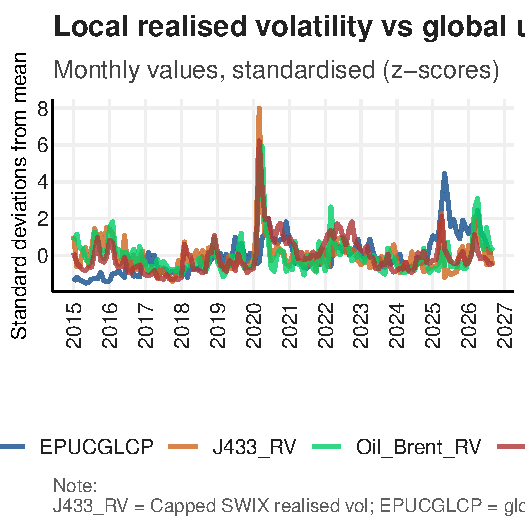
\includegraphics[keepaspectratio,alt={Local realised volatility and global uncertainty (z-scores) }]{Question1_files/figure-latex/FigA6-1.pdf}}
\caption{Local realised volatility and global uncertainty (z-scores)
\label{FigA6}}
\end{figure}

Stratification gives the same ranking (Table \ref{tab:uncstrat}).

\begin{itemize}
\tightlist
\item
  \textbf{When VXEEM is in its top quintile, local volatility is 2.2
  times its level in bottom-quintile months.} The ratio is 1.9 for oil
  volatility and 1.85 for the VIX (all \(p < 0.001\)).
\item
  \textbf{For global policy uncertainty the ratio is only 1.05} (\(p\) =
  0.63).
\end{itemize}

The seminar's concern is therefore partly right. Oil volatility and
global market fear do spill into local equity volatility;
policy-uncertainty indexes, as measured, do not.

\begin{verbatim}
tab_print(Strat_TT %>% rename(Driver = Name, `J433 vol (all)` = J433_RV_All,
                              `J433 vol (High)` = J433_RV_High, `J433 vol (Low)` = J433_RV_Low,
                              `High / Low` = High_vs_Low, `p-value` = p_value),
          caption = "J433 realised volatility when each driver is in its top versus bottom quintile",
          label = "tab:uncstrat", size = "\\scriptsize")
\end{verbatim}

\begin{table}[!htbp]
\centering
\caption{J433 realised volatility when each driver is in its top versus bottom quintile} 
\label{tab:uncstrat}
\begingroup\scriptsize
\begin{tabular}{lrrrrr}
  \hline
Driver & J433 vol (all) & J433 vol (High) & J433 vol (Low) & High / Low & p-value \\ 
  \hline
VXEEM & 0.163 & 0.244 & 0.111 & 2.202 & 0.000 \\ 
  Oil\_Brent\_RV & 0.163 & 0.231 & 0.122 & 1.886 & 0.000 \\ 
  VIX & 0.163 & 0.233 & 0.126 & 1.852 & 0.000 \\ 
  JPMVXYGL & 0.163 & 0.197 & 0.144 & 1.369 & 0.032 \\ 
  MOVE\_Index & 0.163 & 0.189 & 0.139 & 1.354 & 0.051 \\ 
  SAVIUSD & 0.163 & 0.203 & 0.153 & 1.331 & 0.058 \\ 
  EPUCNUSD & 0.163 & 0.201 & 0.163 & 1.230 & 0.179 \\ 
  EPUCGLCP & 0.163 & 0.176 & 0.167 & 1.055 & 0.629 \\ 
   \hline
\end{tabular}
\endgroup
\end{table}

The links have strengthened since 2020 (Table \ref{tab:uncper}).

\begin{itemize}
\tightlist
\item
  \textbf{The VIX:} correlation up from 0.70 to 0.79.
\item
  \textbf{Oil volatility:} up from 0.61 to 0.73.
\item
  \textbf{US policy uncertainty:} turned from negative to positive
  (0.31).
\end{itemize}

Offshore shocks now feed into local volatility more than before.

\begin{verbatim}
tab_print(Cor_By_Period, caption = "Correlation of J433 volatility with each driver, by period",
          label = "tab:uncper")
\end{verbatim}

\begin{table}[!htbp]
\centering
\caption{Correlation of J433 volatility with each driver, by period} 
\label{tab:uncper}
\begingroup\footnotesize
\begin{tabular}{lrr}
  \hline
Name & 2015-2019 & 2020-2026 \\ 
  \hline
EPUCGLCP & -0.327 & 0.019 \\ 
  EPUCNUSD & -0.113 & 0.314 \\ 
  JPMVXYGL & 0.422 & 0.298 \\ 
  MOVE\_Index & 0.425 & 0.060 \\ 
  Oil\_Brent\_RV & 0.606 & 0.733 \\ 
  SAVIUSD & 0.173 & 0.284 \\ 
  VIX & 0.696 & 0.790 \\ 
  VXEEM & 0.759 & 0.767 \\ 
   \hline
\end{tabular}
\endgroup
\end{table}

\subsubsection{Risk and return relative to the Capped
SWIX}\label{risk-and-return-relative-to-the-capped-swix}

SafeCore has outperformed its benchmark without adding volatility, and
with smaller drawdowns (Table \ref{tab:scstats}, Figure \ref{FigB1}).
Over ten years it returned 11.5\% a year against 9.4\% for the Capped
SWIX. Its volatility was virtually identical (14.8\% against 14.7\%) and
its maximum drawdown smaller (27.9\% against 30.2\%), for an information
ratio of 0.52.

\begin{verbatim}
fmxdat::finplot(g_cum, x.date.dist = "1 year", x.date.type = "%Y", x.vert = TRUE)
\end{verbatim}

\begin{figure}
\centering
\pandocbounded{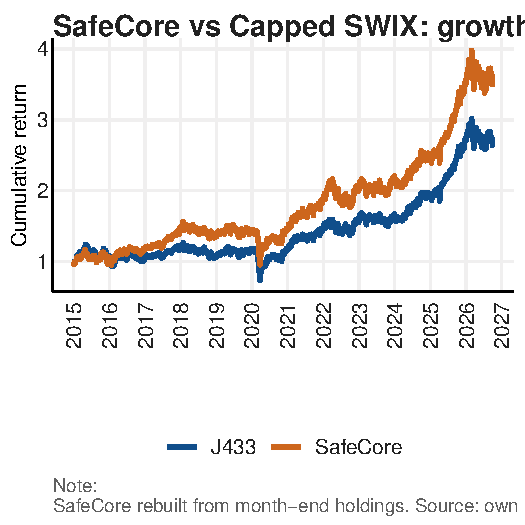
\includegraphics[keepaspectratio,alt={SafeCore versus the Capped SWIX: growth of R1 }]{Question1_files/figure-latex/FigB1-1.pdf}}
\caption{SafeCore versus the Capped SWIX: growth of R1 \label{FigB1}}
\end{figure}

\begin{verbatim}
tab_print(Tab_stats_W, caption = "SafeCore versus the Capped SWIX (monthly returns)",
          label = "tab:scstats", size = "\\scriptsize")
\end{verbatim}

\begin{table}[!htbp]
\centering
\caption{SafeCore versus the Capped SWIX (monthly returns)} 
\label{tab:scstats}
\begingroup\scriptsize
\begin{tabular}{lrrrrrr}
  \hline
Info & SafeCore 3 y & J433 3 y & SafeCore 5 y & J433 5 y & SafeCore 10 y & J433 10 y \\ 
  \hline
Cum Returns & 0.760 & 0.696 & 0.983 & 0.919 & 1.968 & 1.451 \\ 
  Returns (Ann.) & 0.207 & 0.193 & 0.147 & 0.139 & 0.115 & 0.094 \\ 
  Returns Excess (Ann.) & 0.012 & 0.000 & 0.007 & 0.000 & 0.019 & 0.000 \\ 
  SD (Ann.) & 0.134 & 0.128 & 0.151 & 0.137 & 0.148 & 0.147 \\ 
  Max Drawdown & 0.131 & 0.129 & 0.169 & 0.129 & 0.279 & 0.302 \\ 
  Pain Index & 0.028 & 0.026 & 0.041 & 0.032 & 0.047 & 0.046 \\ 
  Tracking Error & 0.032 & 0.000 & 0.037 & 0.000 & 0.041 & 0.000 \\ 
  Information Ratio & 0.460 &  & 0.204 &  & 0.518 &  \\ 
  Beta & 1.018 & 1.000 & 1.072 & 1.000 & 0.971 & 1.000 \\ 
  Beta Bull & 1.072 & 1.000 & 1.029 & 1.000 & 0.904 & 1.000 \\ 
  Beta Bear & 0.838 & 1.000 & 0.917 & 1.000 & 0.870 & 1.000 \\ 
  Up Capture & 1.096 & 1.000 & 1.183 & 1.000 & 1.186 & 1.000 \\ 
  Down Capture & 1.044 & 1.000 & 1.089 & 1.000 & 0.991 & 1.000 \\ 
  Modified CVaR (95\%, monthly) & -0.076 & -0.083 & -0.083 & -0.079 & -0.094 & -0.108 \\ 
   \hline
\end{tabular}
\endgroup
\end{table}

\textbf{Volatility is not managed, and the recent record is mixed.}

\begin{itemize}
\tightlist
\item
  \textbf{Over the last five years} SafeCore was more volatile than the
  benchmark (15.1\% against 13.7\%), with a beta of 1.07, a deeper
  drawdown and a down capture of 1.09.
\item
  \textbf{Over the last three years} it again fell slightly more than
  the market in down months (down capture 1.04).
\item
  \textbf{The rolling one-year beta has risen from about 0.8 in 2016 to
  about one since 2018} (Figure \ref{FigB3}), and rolling volatility has
  tracked the benchmark closely (Figure \ref{FigB2}): SafeCore has
  behaved like the market rather than as a defensive portfolio.
\end{itemize}

\begin{verbatim}
fmxdat::finplot(g_rollsd, x.date.dist = "1 year", x.date.type = "%Y",
                x.vert = TRUE, y.pct = TRUE, y.pct_acc = 1)
\end{verbatim}

\begin{figure}
\centering
\pandocbounded{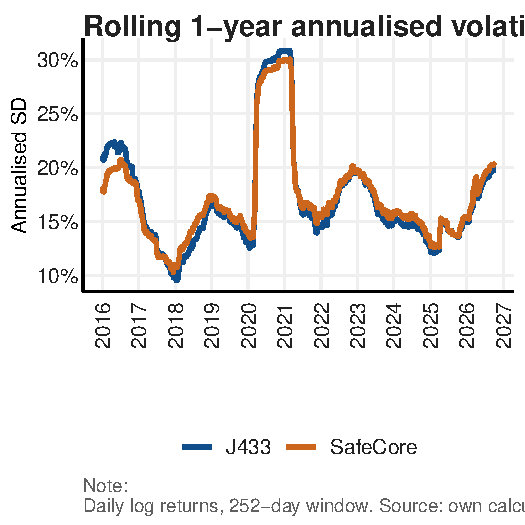
\includegraphics[keepaspectratio,alt={Rolling one-year volatility: SafeCore and J433 }]{Question1_files/figure-latex/FigB2-1.pdf}}
\caption{Rolling one-year volatility: SafeCore and J433 \label{FigB2}}
\end{figure}

\begin{verbatim}
fmxdat::finplot(g_beta, x.date.dist = "1 year", x.date.type = "%Y", x.vert = TRUE)
\end{verbatim}

\begin{figure}
\centering
\pandocbounded{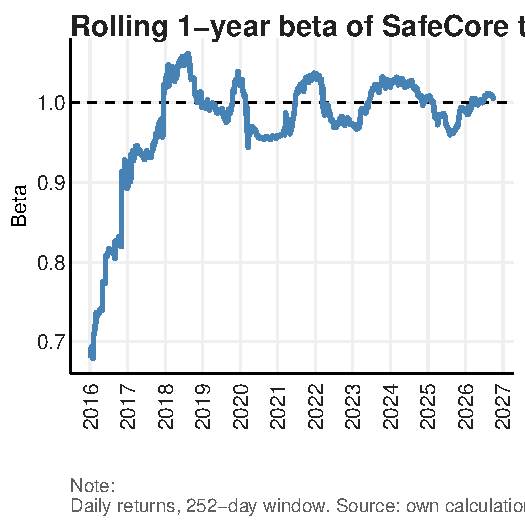
\includegraphics[keepaspectratio,alt={Rolling one-year beta of SafeCore to the Capped SWIX }]{Question1_files/figure-latex/FigB3-1.pdf}}
\caption{Rolling one-year beta of SafeCore to the Capped SWIX
\label{FigB3}}
\end{figure}

Stratification gives a more encouraging picture of stressed markets
(Table \ref{tab:scstrat}).

\begin{itemize}
\tightlist
\item
  \textbf{In the most volatile fifth of months}, SafeCore was slightly
  less volatile than the benchmark (ratio 0.95), and beat it by 0.30\% a
  month, in 66\% of those months.
\item
  \textbf{In the 12 months when the Capped SWIX fell more than 5\%},
  SafeCore lost about 82\% as much (Table \ref{tab:scworst}).
\end{itemize}

Daily downside measures are marginally better than the benchmark's
(Table \ref{tab:scdr}).

\begin{verbatim}
tab_print(Strat_Tab, caption = "SafeCore in high-, low- and normal-volatility months (by J433 volatility)",
          label = "tab:scstrat", size = "\\scriptsize")
\end{verbatim}

\begin{table}[!htbp]
\centering
\caption{SafeCore in high-, low- and normal-volatility months (by J433 volatility)} 
\label{tab:scstrat}
\begingroup\scriptsize
\begin{tabular}{lrrrrrrrr}
  \hline
State & Months & BM\_Vol & SC\_Vol & Vol\_Ratio & BM\_Ret\_Avg & SC\_Ret\_Avg & Excess\_Avg & Hit\_Rate \\ 
  \hline
High vol &   29 & 0.265 & 0.252 & 0.952 & -0.007 & -0.004 & 0.003 & 0.655 \\ 
  Low vol &   29 & 0.097 & 0.103 & 1.064 & 0.012 & 0.012 & 0.001 & 0.517 \\ 
  Normal &   83 & 0.150 & 0.155 & 1.031 & 0.012 & 0.014 & 0.002 & 0.554 \\ 
   \hline
\end{tabular}
\endgroup
\end{table}

\begin{verbatim}
tab_print(Worst_Months, caption = "Months in which the Capped SWIX fell more than 5\\%",
          label = "tab:scworst")
\end{verbatim}

\begin{table}[!htbp]
\centering
\caption{Months in which the Capped SWIX fell more than 5\%} 
\label{tab:scworst}
\begingroup\footnotesize
\begin{tabular}{rrrr}
  \hline
Months & BM\_Ret\_Avg & SC\_Ret\_Avg & Capture \\ 
  \hline
  12 & -0.078 & -0.063 & 0.816 \\ 
   \hline
\end{tabular}
\endgroup
\end{table}

\begin{verbatim}
tab_print(DR_Tab_T, caption = "Downside risk on daily returns", label = "tab:scdr", digits = 4)
\end{verbatim}

\begin{table}[!htbp]
\centering
\caption{Downside risk on daily returns} 
\label{tab:scdr}
\begingroup\footnotesize
\begin{tabular}{lrr}
  \hline
Measure & SafeCore & J433 \\ 
  \hline
Semi Deviation & 0.0081 & 0.0082 \\ 
  Gain Deviation & 0.0073 & 0.0075 \\ 
  Loss Deviation & 0.0081 & 0.0084 \\ 
  Downside Deviation (MAR=0\%) & 0.0079 & 0.0080 \\ 
  Downside Deviation (Rf=0\%) & 0.0079 & 0.0080 \\ 
  Downside Deviation (0\%) & 0.0079 & 0.0080 \\ 
  Maximum Drawdown & 0.3908 & 0.4166 \\ 
  Historical VaR (95\%) & -0.0166 & -0.0165 \\ 
  Historical ES (95\%) & -0.0252 & -0.0258 \\ 
  Modified VaR (95\%) & -0.0180 & -0.0179 \\ 
  Modified ES (95\%) & -0.0327 & -0.0348 \\ 
   \hline
\end{tabular}
\endgroup
\end{table}

\textbf{A dedicated low-volatility tilt offers more protection.} Since
the Low Volatility index starts in 2024, SafeCore and J433 had almost
identical returns, while the Low Volatility index was clearly less
volatile (14.4\% against 16.4\% for SafeCore) and had a smaller drawdown
(Table \ref{tab:sclv}). It also earned less in the strong 2025--26
market.

\begin{verbatim}
tab_print(LV_Tab_T, caption = "SafeCore, J433 and the Low Volatility index since 2024 (daily returns)",
          label = "tab:sclv")
\end{verbatim}

\begin{table}[!htbp]
\centering
\caption{SafeCore, J433 and the Low Volatility index since 2024 (daily returns)} 
\label{tab:sclv}
\begingroup\footnotesize
\begin{tabular}{lrrr}
  \hline
Measure & SafeCore & J433 & LowVol \\ 
  \hline
Annualized Return & 0.180 & 0.179 & 0.137 \\ 
  Annualized Std Dev & 0.164 & 0.159 & 0.144 \\ 
  Annualized Sharpe (Rf=0\%) & 1.099 & 1.125 & 0.951 \\ 
  Worst Drawdown & 0.152 & 0.141 & 0.131 \\ 
   \hline
\end{tabular}
\endgroup
\end{table}

\subsubsection{Where does SafeCore's volatility come
from?}\label{where-does-safecores-volatility-come-from}

SafeCore's risk is now concentrated in a few gold miners (Table
\ref{tab:es}, Table \ref{tab:rvw}).

\begin{itemize}
\tightlist
\item
  \textbf{Expected Shortfall:} over the last two years, Gold Fields and
  AngloGold Ashanti together account for about 36\% of SafeCore's
  Expected Shortfall.
\item
  \textbf{Current holdings:} these two stocks are about 20\% of the
  portfolio by weight but about 40\% of its volatility. Each contributes
  about twice as much risk as its weight.
\end{itemize}

\begin{verbatim}
tab_print(ES_Top %>% rename(`Contribution to ES` = Risk_Contrib),
          caption = "Largest contributions to Expected Shortfall, last two years", label = "tab:es")
\end{verbatim}

\begin{table}[!htbp]
\centering
\caption{Largest contributions to Expected Shortfall, last two years} 
\label{tab:es}
\begingroup\footnotesize
\begin{tabular}{lrl}
  \hline
Tickers & Contribution to ES & Window \\ 
  \hline
GFI & 0.179 & Last 2 years \\ 
  ANG & 0.179 & Last 2 years \\ 
  SSW & 0.103 & Last 2 years \\ 
  HAR & 0.068 & Last 2 years \\ 
  SBK & 0.067 & Last 2 years \\ 
  MTN & 0.056 & Last 2 years \\ 
  ABG & 0.050 & Last 2 years \\ 
  FSR & 0.038 & Last 2 years \\ 
  OMU & 0.029 & Last 2 years \\ 
  BHG & 0.026 & Last 2 years \\ 
   \hline
\end{tabular}
\endgroup
\end{table}

\begin{verbatim}
tab_print(Risk_vs_Weight %>% head(12) %>%
            rename(`Share of volatility` = SD_Contrib, `Risk / weight` = Risk_per_Weight),
          caption = "Current holdings: weight versus contribution to volatility (top 12)",
          label = "tab:rvw")
\end{verbatim}

\begin{table}[!htbp]
\centering
\caption{Current holdings: weight versus contribution to volatility (top 12)} 
\label{tab:rvw}
\begingroup\footnotesize
\begin{tabular}{lrrlr}
  \hline
Tickers & Weight & Share of volatility & Sector & Risk / weight \\ 
  \hline
ANG & 0.120 & 0.249 & Resources & 2.077 \\ 
  GFI & 0.075 & 0.156 & Resources & 2.085 \\ 
  VAL & 0.044 & 0.094 & Resources & 2.131 \\ 
  MTN & 0.088 & 0.072 & Industrials & 0.814 \\ 
  SBK & 0.101 & 0.067 & Financials & 0.658 \\ 
  PAN & 0.028 & 0.049 & Resources & 1.766 \\ 
  ABG & 0.072 & 0.046 & Financials & 0.633 \\ 
  FSR & 0.051 & 0.034 & Financials & 0.661 \\ 
  BHG & 0.047 & 0.033 & Resources & 0.710 \\ 
  SOL & 0.048 & 0.026 & Resources & 0.529 \\ 
  NPN & 0.047 & 0.023 & Industrials & 0.493 \\ 
  SSW & 0.010 & 0.023 & Resources & 2.281 \\ 
   \hline
\end{tabular}
\endgroup
\end{table}

By sector, Resources make up about 40\% of the weight but 65\% of the
volatility (Table \ref{tab:secrisk}, Figure \ref{FigB4}). Their share of
risk has risen sharply over time, from about 10--20\% in 2015--19 to
65\% in 2026 (Figure \ref{FigB5}, Table \ref{tab:yearrisk}).

\begin{verbatim}
tab_print(Sector_Risk %>% rename(`Share of weight` = Weight, `Share of volatility` = SD_Contrib),
          caption = "Share of weight versus share of volatility by sector (current holdings)",
          label = "tab:secrisk")
\end{verbatim}

\begin{table}[!htbp]
\centering
\caption{Share of weight versus share of volatility by sector (current holdings)} 
\label{tab:secrisk}
\begingroup\footnotesize
\begin{tabular}{lrr}
  \hline
Sector & Share of weight & Share of volatility \\ 
  \hline
Resources & 0.401 & 0.649 \\ 
  Financials & 0.313 & 0.195 \\ 
  Industrials & 0.260 & 0.147 \\ 
  Property & 0.025 & 0.009 \\ 
   \hline
\end{tabular}
\endgroup
\end{table}

\begin{verbatim}
fmxdat::finplot(g_sector, y.pct = TRUE, y.pct_acc = 1)
\end{verbatim}

\begin{figure}
\centering
\pandocbounded{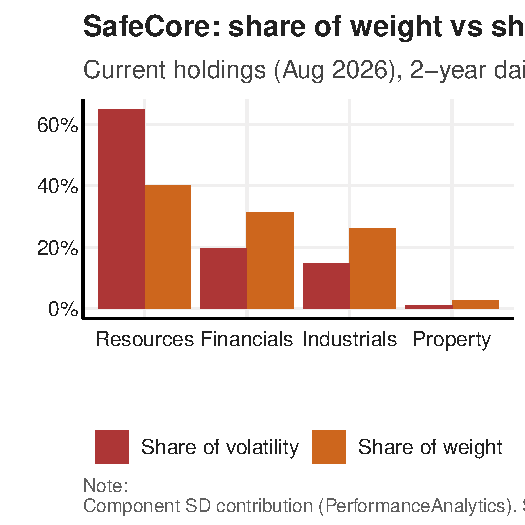
\includegraphics[keepaspectratio,alt={Share of weight versus share of volatility by sector }]{Question1_files/figure-latex/FigB4-1.pdf}}
\caption{Share of weight versus share of volatility by sector
\label{FigB4}}
\end{figure}

\begin{verbatim}
fmxdat::finplot(g_yearly, y.pct = TRUE, y.pct_acc = 1)
\end{verbatim}

\begin{figure}
\centering
\pandocbounded{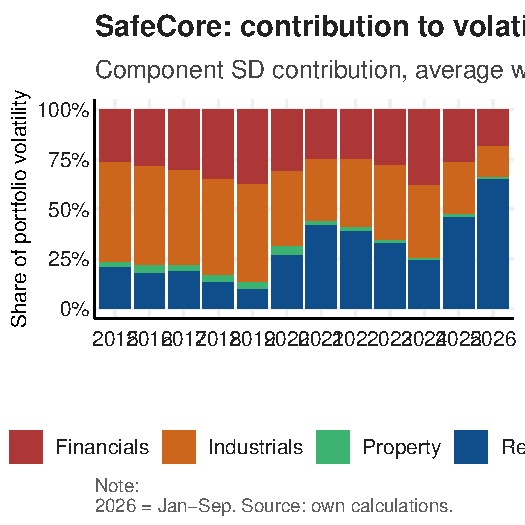
\includegraphics[keepaspectratio,alt={Contribution to volatility by sector over time }]{Question1_files/figure-latex/FigB5-1.pdf}}
\caption{Contribution to volatility by sector over time \label{FigB5}}
\end{figure}

\begin{verbatim}
tab_print(Yearly_Risk_Tab %>% mutate(Year = as.character(Year)),
          caption = "Contribution to volatility by sector and year", label = "tab:yearrisk",
          size = "\\scriptsize")
\end{verbatim}

\begin{table}[!htbp]
\centering
\caption{Contribution to volatility by sector and year} 
\label{tab:yearrisk}
\begingroup\scriptsize
\begin{tabular}{lrrrr}
  \hline
Year & Financials & Industrials & Property & Resources \\ 
  \hline
2015 & 0.264 & 0.506 & 0.021 & 0.209 \\ 
  2016 & 0.286 & 0.498 & 0.040 & 0.177 \\ 
  2017 & 0.306 & 0.478 & 0.028 & 0.188 \\ 
  2018 & 0.352 & 0.481 & 0.035 & 0.133 \\ 
  2019 & 0.376 & 0.492 & 0.034 & 0.098 \\ 
  2020 & 0.312 & 0.378 & 0.040 & 0.270 \\ 
  2021 & 0.252 & 0.313 & 0.016 & 0.420 \\ 
  2022 & 0.249 & 0.344 & 0.019 & 0.388 \\ 
  2023 & 0.279 & 0.377 & 0.016 & 0.328 \\ 
  2024 & 0.382 & 0.365 & 0.013 & 0.240 \\ 
  2025 & 0.265 & 0.265 & 0.013 & 0.457 \\ 
  2026 & 0.184 & 0.157 & 0.009 & 0.651 \\ 
   \hline
\end{tabular}
\endgroup
\end{table}

Part of this is a deliberate bet: SafeCore is overweight Resources
relative to the Capped SWIX, mainly through AngloGold Ashanti (Table
\ref{tab:active}). It is also overweight the large banks and MTN, and
underweight Industrials and Property.

\begin{verbatim}
tab_print(Sector_Active, caption = "SafeCore versus Capped SWIX sector weights (latest month)",
          label = "tab:active")
\end{verbatim}

\begin{table}[!htbp]
\centering
\caption{SafeCore versus Capped SWIX sector weights (latest month)} 
\label{tab:active}
\begingroup\footnotesize
\begin{tabular}{lrrr}
  \hline
Sector & SafeCore & CappedSWIX & Active \\ 
  \hline
Resources & 0.401 & 0.348 & 0.054 \\ 
  Financials & 0.313 & 0.289 & 0.025 \\ 
  Unclassified & 0.000 & 0.007 & -0.007 \\ 
  Property & 0.025 & 0.045 & -0.019 \\ 
  Industrials & 0.260 & 0.312 & -0.052 \\ 
   \hline
\end{tabular}
\endgroup
\end{table}

\subsubsection{Factor exposures}\label{factor-exposures}

Our momentum score agrees broadly with the third party's: the average
monthly rank correlation is 0.60 (Table \ref{tab:rankcor}, Figure
\ref{FigB6}). The remaining differences reflect construction choices,
such as the look-back window, which the third party does not disclose.

Our low-volatility score, however, does not line up with the third
party's ``Volatility Sensitivity''. A low-volatility stock should have
low sensitivity, so the correlation should be strongly negative. Instead
it averages \(+0.11\). Volatility Sensitivity is also essentially
uncorrelated with realised volatility (\(-0.11\)) and with beta (0.00)
(Table \ref{tab:volsens}). It is therefore not a volatility measure, so
we use our own price-based score for low volatility.

\begin{verbatim}
tab_print(Rank_Cor_T, caption = "Monthly Spearman rank correlation: own versus third-party scores",
          label = "tab:rankcor")
\end{verbatim}

\begin{table}[!htbp]
\centering
\caption{Monthly Spearman rank correlation: own versus third-party scores} 
\label{tab:rankcor}
\begingroup\footnotesize
\begin{tabular}{lrrr}
  \hline
Comparison & Mean & Min & Max \\ 
  \hline
Own momentum vs third-party momentum & 0.602 & 0.031 & 0.909 \\ 
  Own low-vol vs third-party volatility sensitivity & 0.108 & -0.160 & 0.412 \\ 
   \hline
\end{tabular}
\endgroup
\end{table}

\begin{verbatim}
tab_print(VolSens_Check, caption = "What does Volatility Sensitivity track? (average monthly rank correlation)",
          label = "tab:volsens")
\end{verbatim}

\begin{table}[!htbp]
\centering
\caption{What does Volatility Sensitivity track? (average monthly rank correlation)} 
\label{tab:volsens}
\begingroup\footnotesize
\begin{tabular}{rr}
  \hline
VolSens\_vs\_RealisedVol & VolSens\_vs\_Beta \\ 
  \hline
-0.108 & -0.003 \\ 
   \hline
\end{tabular}
\endgroup
\end{table}

\begin{verbatim}
fmxdat::finplot(g_cor, x.date.dist = "1 year", x.date.type = "%Y", x.vert = TRUE)
\end{verbatim}

\begin{figure}
\centering
\pandocbounded{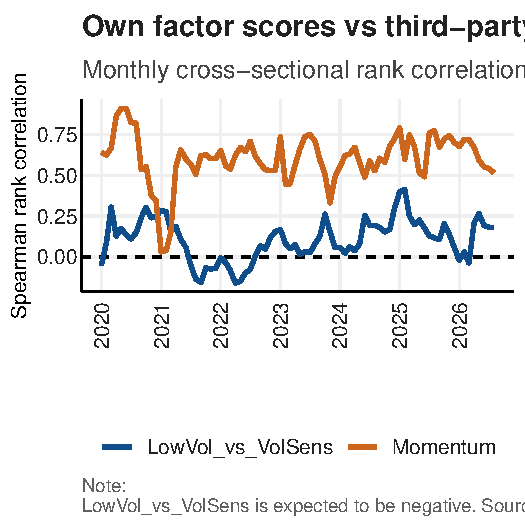
\includegraphics[keepaspectratio,alt={Own versus third-party factor scores: monthly rank correlation }]{Question1_files/figure-latex/FigB6-1.pdf}}
\caption{Own versus third-party factor scores: monthly rank correlation
\label{FigB6}}
\end{figure}

SafeCore's active tilts are towards momentum, earnings quality and
value, not low volatility (Table \ref{tab:exp}, Figure \ref{FigB7}).

\begin{itemize}
\tightlist
\item
  \textbf{Momentum is the largest tilt:} +0.33 standard deviations in
  the latest month.
\item
  \textbf{Earnings quality} is +0.15 and \textbf{value} +0.13.
\item
  \textbf{Low volatility is slightly negative} (\(-0.09\)): SafeCore
  currently leans towards more volatile stocks, consistent with its
  gold-miner overweight.
\end{itemize}

\begin{verbatim}
tab_print(Exp_Tab %>% rename(`Avg. 2020-26` = Active_Avg_2020_26, `Last 12 months` = Active_Last_12m,
                             Latest = Active_Latest),
          caption = "SafeCore's active factor exposure relative to the Capped SWIX (z-score units)",
          label = "tab:exp")
\end{verbatim}

\begin{table}[!htbp]
\centering
\caption{SafeCore's active factor exposure relative to the Capped SWIX (z-score units)} 
\label{tab:exp}
\begingroup\footnotesize
\begin{tabular}{lrrr}
  \hline
Factor & Avg. 2020-26 & Last 12 months & Latest \\ 
  \hline
Momentum & 0.105 & 0.213 & 0.325 \\ 
  Earnings Quality & 0.146 & 0.204 & 0.149 \\ 
  Value & 0.085 & 0.100 & 0.126 \\ 
  Growth & 0.060 & 0.013 & 0.052 \\ 
  Own\_Momentum & 0.066 & 0.148 & -0.012 \\ 
  Own\_LowVol & 0.008 & -0.058 & -0.085 \\ 
  Volatility Sensitivity & 0.007 & -0.054 & -0.135 \\ 
   \hline
\end{tabular}
\endgroup
\end{table}

\begin{verbatim}
fmxdat::finplot(g_exp, x.date.dist = "2 years", x.date.type = "%Y", x.vert = TRUE)
\end{verbatim}

\begin{figure}
\centering
\pandocbounded{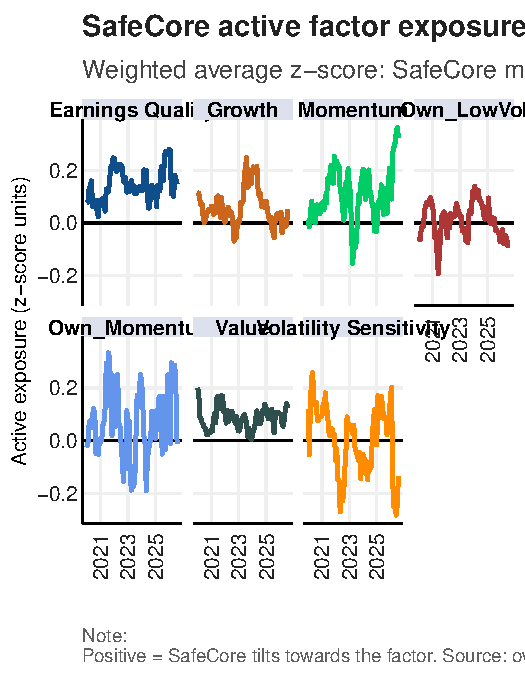
\includegraphics[keepaspectratio,alt={SafeCore's active factor exposure over time }]{Question1_files/figure-latex/FigB7-1.pdf}}
\caption{SafeCore's active factor exposure over time \label{FigB7}}
\end{figure}

The composite scores put these tilts in context (Table \ref{tab:purity},
Figure \ref{FigB8}).

\begin{itemize}
\tightlist
\item
  \textbf{On every strategy, SafeCore sits only 3--14\% of the way from
  the benchmark to a pure strategy portfolio.} The strongest are
  quality-growth and momentum.
\item
  \textbf{The defensive composite is now close to zero.}
\end{itemize}

SafeCore is therefore a mildly tilted, benchmark-like portfolio, with no
meaningful defensive or low-volatility ballast.

\begin{verbatim}
tab_print(Strat_Avg, caption = "Composite strategy scores: SafeCore, benchmark and pure strategy (average 2020-26)",
          label = "tab:purity")
\end{verbatim}

\begin{table}[!htbp]
\centering
\caption{Composite strategy scores: SafeCore, benchmark and pure strategy (average 2020-26)} 
\label{tab:purity}
\begingroup\footnotesize
\begin{tabular}{lrrrr}
  \hline
Strategy & SafeCore & CappedSWIX & Top\_Quintile\_EW & Purity \\ 
  \hline
Quality\_Growth & 0.245 & 0.080 & 1.428 & 0.124 \\ 
  Defensive & 0.066 & -0.074 & 1.298 & 0.101 \\ 
  Momentum\_C & 0.302 & 0.202 & 1.368 & 0.088 \\ 
  Value\_C & -0.406 & -0.501 & 1.500 & 0.048 \\ 
   \hline
\end{tabular}
\endgroup
\end{table}

\begin{verbatim}
fmxdat::finplot(g_strat, x.date.dist = "1 year", x.date.type = "%Y", x.vert = TRUE)
\end{verbatim}

\begin{figure}
\centering
\pandocbounded{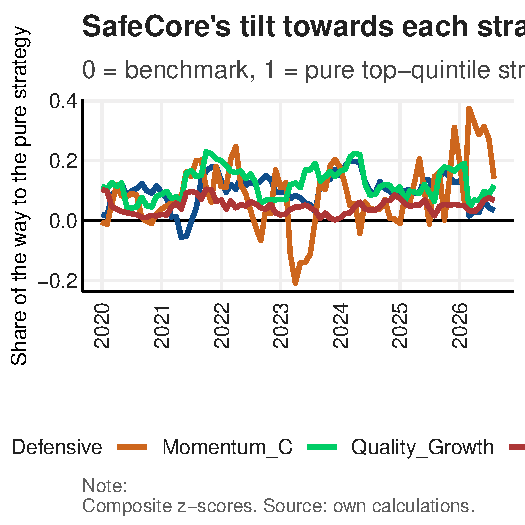
\includegraphics[keepaspectratio,alt={SafeCore's tilt towards each strategy (purity) }]{Question1_files/figure-latex/FigB8-1.pdf}}
\caption{SafeCore's tilt towards each strategy (purity) \label{FigB8}}
\end{figure}

\subsection{Part C: Alpha opportunity since
2020}\label{part-c-alpha-opportunity-since-2020}

Weighted dispersion is used as the main measure, for two reasons.

\begin{itemize}
\tightlist
\item
  \textbf{It follows the question's formula}, measuring spread around
  the Capped SWIX.
\item
  \textbf{It is the spread that matters to a benchmark-aware manager},
  since that manager can only profit from stocks large enough to hold.
\end{itemize}

The unweighted measure is dominated by small, illiquid names. It also
fell after 2020 partly because the index shrank from about 155 to 121
stocks (Table \ref{tab:disp}, Figure \ref{FigC1}).

Weighted dispersion peaked in 2020 (19.6\%) and has stayed above its
2015--19 level since (14.4\% and 13.8\%).

\begin{verbatim}
tab_print(Disp_Periods, caption = "Average 12-week cross-sectional dispersion by period",
          label = "tab:disp")
\end{verbatim}

\begin{table}[!htbp]
\centering
\caption{Average 12-week cross-sectional dispersion by period} 
\label{tab:disp}
\begingroup\footnotesize
\begin{tabular}{lrrr}
  \hline
Period & Weighted & Unweighted & Avg\_Stocks \\ 
  \hline
1. 2015-2019 & 0.128 & 0.160 & 154.508 \\ 
  2. 2020 & 0.196 & 0.229 & 142.943 \\ 
  3. 2021-2023 & 0.144 & 0.155 & 132.026 \\ 
  4. 2024-2026 & 0.138 & 0.139 & 120.767 \\ 
   \hline
\end{tabular}
\endgroup
\end{table}

\begin{verbatim}
fmxdat::finplot(g_disp, x.date.dist = "1 year", x.date.type = "%Y",
                x.vert = TRUE, y.pct = TRUE, y.pct_acc = 1)
\end{verbatim}

\begin{verbatim}
## Warning: Removed 22 rows containing missing values or values outside the scale range
## (`geom_line()`).
\end{verbatim}

\begin{figure}
\centering
\pandocbounded{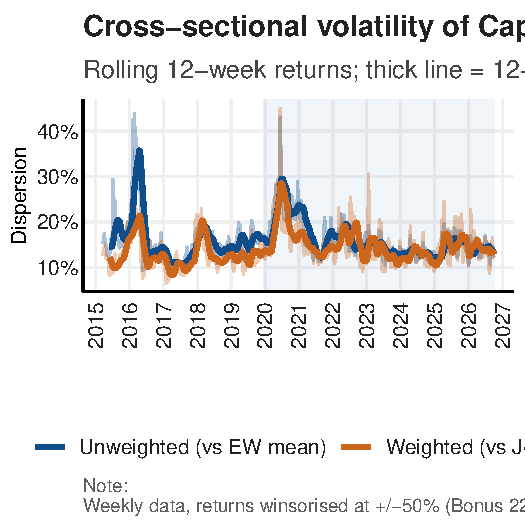
\includegraphics[keepaspectratio,alt={Cross-sectional dispersion of Capped SWIX constituents }]{Question1_files/figure-latex/FigC1-1.pdf}}
\caption{Cross-sectional dispersion of Capped SWIX constituents
\label{FigC1}}
\end{figure}

Correlation among the 40 largest stocks has fallen to its lowest level
in the sample (Table \ref{tab:corr}, Figure \ref{FigC2}). The average
pairwise correlation is 0.20 in 2024--26, against 0.26 in 2015--19, and
the first principal component explains 29\% of the variance, against
35\%.

\begin{verbatim}
tab_print(Corr_Periods %>% rename(`Avg. correlation` = Avg_Corr, `Weighted avg. correlation` = Avg_Corr_W,
                                  `PC1 share` = PC1_Share),
          caption = "Co-movement among the 40 largest stocks by period", label = "tab:corr")
\end{verbatim}

\begin{table}[!htbp]
\centering
\caption{Co-movement among the 40 largest stocks by period} 
\label{tab:corr}
\begingroup\footnotesize
\begin{tabular}{lrrr}
  \hline
Period & Avg. correlation & Weighted avg. correlation & PC1 share \\ 
  \hline
1. 2015-2019 & 0.261 & 0.265 & 0.348 \\ 
  2. 2020 & 0.323 & 0.305 & 0.393 \\ 
  3. 2021-2023 & 0.242 & 0.230 & 0.310 \\ 
  4. 2024-2026 & 0.203 & 0.205 & 0.289 \\ 
   \hline
\end{tabular}
\endgroup
\end{table}

\begin{verbatim}
fmxdat::finplot(g_corr, x.date.dist = "1 year", x.date.type = "%Y",
                x.vert = TRUE, y.pct = TRUE, y.pct_acc = 1)
\end{verbatim}

\begin{figure}
\centering
\pandocbounded{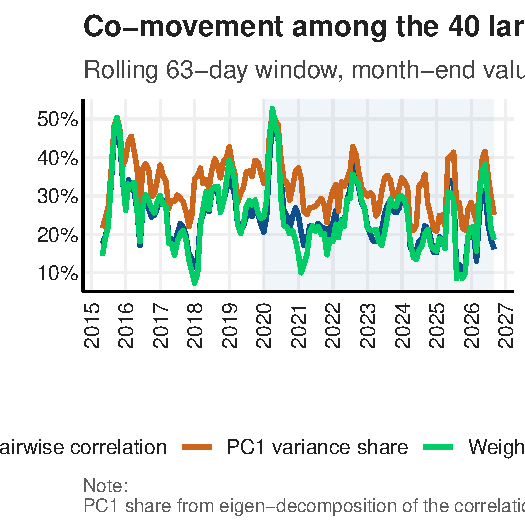
\includegraphics[keepaspectratio,alt={Co-movement among the 40 largest Capped SWIX stocks }]{Question1_files/figure-latex/FigC2-1.pdf}}
\caption{Co-movement among the 40 largest Capped SWIX stocks
\label{FigC2}}
\end{figure}

Together, these measures show that the alpha opportunity has improved
since 2020 (Figure \ref{FigC3}).

\begin{itemize}
\tightlist
\item
  \textbf{2020 was a false opportunity.} Dispersion was high, but so was
  correlation: the whole market moved together, and the spread came from
  volatility rather than stock-specific stories.
\item
  \textbf{Since 2021 the market has moved towards the best region for
  stock pickers}: dispersion above its pre-2020 level, with lower
  correlation.
\item
  \textbf{The pattern recurred briefly in 2025 and 2026}, when
  correlation jumped during the global shocks identified in Part A.
\end{itemize}

\begin{verbatim}
fmxdat::finplot(g_opp, x.pct = TRUE, x.pct_acc = 1, y.pct = TRUE, y.pct_acc = 1)
\end{verbatim}

\begin{figure}
\centering
\pandocbounded{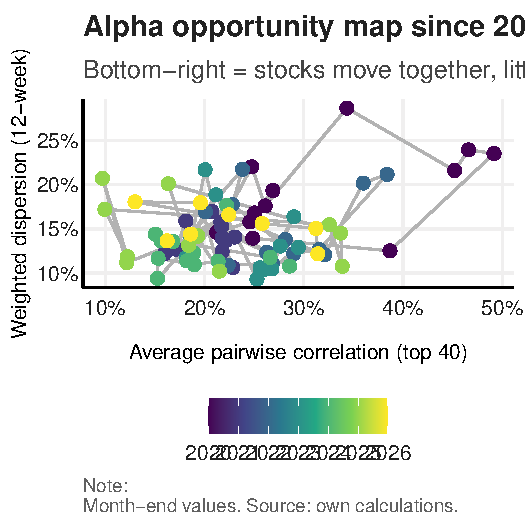
\includegraphics[keepaspectratio,alt={Alpha opportunity map since 2020: dispersion against correlation }]{Question1_files/figure-latex/FigC3-1.pdf}}
\caption{Alpha opportunity map since 2020: dispersion against
correlation \label{FigC3}}
\end{figure}

Global macro conditions shape the opportunity set (Tables
\ref{tab:macrocor} and \ref{tab:macrostrat}).

\begin{itemize}
\tightlist
\item
  \textbf{Global fear raises dispersion and correlation together.} When
  the VIX, EM implied volatility, oil volatility or rand volatility is
  in its top quintile:

  \begin{itemize}
  \tightlist
  \item
    dispersion is 1.3--1.4 times higher than in bottom-quintile months;
  \item
    average correlation is about 0.10 higher.
  \end{itemize}

  The extra spread comes with stocks moving together, so it is harder to
  exploit.
\item
  \textbf{Global policy uncertainty is the exception.} It raises
  dispersion (1.21 times) with almost no rise in correlation: the only
  ``good'' dispersion among the drivers.
\item
  \textbf{Bond-market volatility (MOVE) slightly reduces dispersion.}
\end{itemize}

\begin{verbatim}
tab_print(Macro_Cor %>% rename(Driver = Name, Dispersion = Dispersion_W, `Avg. correlation` = Avg_Corr,
                               `PC1 share` = PC1_Share),
          caption = "Correlation of monthly alpha-opportunity measures with global drivers (since 2020)",
          label = "tab:macrocor")
\end{verbatim}

\begin{table}[!htbp]
\centering
\caption{Correlation of monthly alpha-opportunity measures with global drivers (since 2020)} 
\label{tab:macrocor}
\begingroup\footnotesize
\begin{tabular}{lrrr}
  \hline
Driver & Dispersion & Avg. correlation & PC1 share \\ 
  \hline
VIX & 0.538 & 0.613 & 0.560 \\ 
  VXEEM & 0.468 & 0.529 & 0.532 \\ 
  Oil\_Brent\_RV & 0.457 & 0.605 & 0.600 \\ 
  EPUCGLCP & 0.212 & 0.144 & 0.253 \\ 
  SAVIUSD & 0.200 & 0.362 & 0.365 \\ 
  JPMVXYGL & 0.193 & 0.365 & 0.295 \\ 
  MOVE\_Index & -0.205 & 0.130 & 0.043 \\ 
   \hline
\end{tabular}
\endgroup
\end{table}

\begin{verbatim}
tab_print(Strat %>% rename(Driver = Name) %>%
            select(Driver, `Disp. High` = Dispersion_W_High, `Disp. Low` = Dispersion_W_Low,
                   `Disp. High/Low` = Disp_High_vs_Low, `Corr. High` = Avg_Corr_High,
                   `Corr. Low` = Avg_Corr_Low, `Corr. High - Low` = Corr_High_minus_Low),
          caption = "Dispersion and correlation when each driver is in its top versus bottom quintile (since 2020)",
          label = "tab:macrostrat", size = "\\scriptsize")
\end{verbatim}

\begin{table}[!htbp]
\centering
\caption{Dispersion and correlation when each driver is in its top versus bottom quintile (since 2020)} 
\label{tab:macrostrat}
\begingroup\scriptsize
\begin{tabular}{lrrrrrr}
  \hline
Driver & Disp. High & Disp. Low & Disp. High/Low & Corr. High & Corr. Low & Corr. High - Low \\ 
  \hline
VIX & 0.179 & 0.125 & 1.432 & 0.319 & 0.215 & 0.103 \\ 
  VXEEM & 0.172 & 0.133 & 1.290 & 0.304 & 0.196 & 0.108 \\ 
  Oil\_Brent\_RV & 0.185 & 0.144 & 1.290 & 0.308 & 0.211 & 0.097 \\ 
  SAVIUSD & 0.185 & 0.146 & 1.265 & 0.303 & 0.199 & 0.104 \\ 
  EPUCGLCP & 0.162 & 0.134 & 1.211 & 0.231 & 0.225 & 0.006 \\ 
  JPMVXYGL & 0.156 & 0.136 & 1.147 & 0.294 & 0.218 & 0.076 \\ 
  MOVE\_Index & 0.148 & 0.170 & 0.870 & 0.283 & 0.249 & 0.034 \\ 
   \hline
\end{tabular}
\endgroup
\end{table}

\section{\texorpdfstring{Model summary
\label{Summary}}{Model summary }}\label{model-summary}

\begin{verbatim}
Summary_Tab <- tibble(
  Question = c("A: Has local vol increased?", "A: Does it mirror global?", "A: GJR-GARCH",
               "A: VIX in variance equation", "A: DCC correlation", "A: Offshore drivers",
               "B: SafeCore vs J433", "B: Sources of risk", "B: Factor tilts",
               "C: Alpha opportunity", "C: Macro link"),
  Finding = c("Not structurally; but up sharply in 2026 (20.7% vs 15.0%)",
              "Yes - closest to EM; well above developed markets",
              "Strong leverage effect (gamma > 0, alpha close to 0); half-life about 20 days",
              "Positive and significant: global fear raises local variance",
              "Stable long-run level (about 0.65-0.69), spikes in crises",
              "VXEEM, VIX and oil vol matter; policy-uncertainty indexes do not",
              "Higher return, same vol, smaller drawdown; beta about 1 since 2018",
              "Gold miners: about 20% of weight but 40% of vol; Resources 65% of vol",
              "Momentum, quality, value; no low-vol ballast",
              "Improved since 2020: higher dispersion, lowest correlation",
              "Global fear raises dispersion and correlation together")
)
print(xtable::xtable(Summary_Tab, caption = "Summary of findings", label = "tab:summary",
                     align = c("l", "p{4.2cm}", "p{10cm}")),
      include.rownames = FALSE, comment = FALSE, table.placement = "!htbp",
      caption.placement = "top", size = "\\scriptsize")
\end{verbatim}

\begin{table}[!htbp]
\centering
\caption{Summary of findings} 
\label{tab:summary}
\begingroup\scriptsize
\begin{tabular}{p{4.2cm}p{10cm}}
  \hline
Question & Finding \\ 
  \hline
A: Has local vol increased? & Not structurally; but up sharply in 2026 (20.7\% vs 15.0\%) \\ 
  A: Does it mirror global? & Yes - closest to EM; well above developed markets \\ 
  A: GJR-GARCH & Strong leverage effect (gamma $>$ 0, alpha close to 0); half-life about 20 days \\ 
  A: VIX in variance equation & Positive and significant: global fear raises local variance \\ 
  A: DCC correlation & Stable long-run level (about 0.65-0.69), spikes in crises \\ 
  A: Offshore drivers & VXEEM, VIX and oil vol matter; policy-uncertainty indexes do not \\ 
  B: SafeCore vs J433 & Higher return, same vol, smaller drawdown; beta about 1 since 2018 \\ 
  B: Sources of risk & Gold miners: about 20\% of weight but 40\% of vol; Resources 65\% of vol \\ 
  B: Factor tilts & Momentum, quality, value; no low-vol ballast \\ 
  C: Alpha opportunity & Improved since 2020: higher dispersion, lowest correlation \\ 
  C: Macro link & Global fear raises dispersion and correlation together \\ 
   \hline
\end{tabular}
\endgroup
\end{table}

Table \ref{tab:summary} summarises the findings.

\textbf{Part A:}

\begin{itemize}
\tightlist
\item
  Local volatility has not risen structurally since 2015, but it has
  jumped in 2026 and moves closely with global, and especially
  emerging-market, volatility.
\item
  The GJR-GARCH models show that volatility responds mainly to bad news.
\item
  The VIX raises local conditional variance directly.
\item
  DCC correlations with global markets rise sharply in crises.
\item
  Offshore market fear and oil volatility separate calm from volatile
  local months; policy-uncertainty indexes do not.
\end{itemize}

\textbf{Part B:}

\begin{itemize}
\tightlist
\item
  SafeCore has rewarded investors, with higher returns at similar
  volatility and smaller long-run drawdowns, and has held up reasonably
  in the worst months.
\item
  It was not built with volatility in mind, and it shows: beta has risen
  to about one, its risk is concentrated in gold miners, and its factor
  tilts do not include low volatility.
\end{itemize}

\textbf{Part C:} the opportunity for stock selection has improved since
2020. However, the global shocks that raise local volatility also raise
correlation, which reduces the benefit of stock picking exactly when
volatility is highest.

\textbf{Implications for the team.} The case for building a risk ballast
into SafeCore is supported. Three steps would help:

\begin{enumerate}
\def\labelenumi{\arabic{enumi}.}
\tightlist
\item
  \textbf{Monitor and cap the risk contribution of the gold miners},
  rather than their weight.
\item
  \textbf{Add an explicit low-volatility or defensive tilt}, measured
  with price-based scores, since the third-party volatility score does
  not capture volatility.
\item
  \textbf{Treat spikes in the VIX, EM implied volatility and oil
  volatility as early-warning signals for local risk.}
\end{enumerate}

\textbf{Limitations:}

\begin{itemize}
\tightlist
\item
  the short history of the Low Volatility index;
\item
  the monthly frequency of the policy-uncertainty indexes;
\item
  the modest number of extreme months in each stratification;
\item
  currency effects: global indexes are in US dollars, local ones in
  rand.
\end{itemize}

\newpage

\section*{References}\label{references}
\addcontentsline{toc}{section}{References}

\protect\phantomsection\label{refs}

\bibliography{Tex/ref}





\end{document}
